\documentclass{article}
\usepackage[utf8]{inputenc}
\usepackage{amssymb}
\usepackage{amsmath}
\usepackage{float}
\usepackage{epstopdf}
\usepackage{moreverb}
\usepackage{multicol}
\usepackage{listings}
\usepackage{mathrsfs}
\usepackage{graphicx}
\usepackage{cite}
\usepackage{tabularx}
\usepackage{listings}
\newcommand{\R}{\mathbb{R}}
\newcommand{\overbar}[1]{\mkern 1.5mu\overline{\mkern-1.5mu#1\mkern-1.5mu}\mkern 1.5mu}




\bibliographystyle{plain}
\title{APPM 5720 Homework 3}
\author{Wil Boshell, Fortino Garcia, Alex Rybchuk, Parth Thakkar}
\date{February 12, 2018}


\begin{document}
%\def\code#1{\texttt{#1}}

\maketitle

\section{Preliminaries}
Consider a grid with $N +1$ grid points $x_L = x_0 < x_1 < x_2 < \dots < x_N = x_R$, defining $N$ elements $\Omega_i =  \{x \in [ x_{i-1}, x_i ] \} $, $i=1,\dots,N$. We seek to approximate a function $f(x)$ on $x \in \left[ x_L, x_R \right]$ by $L_2$ projection onto the space of element-wise Legendre polynomials of degree $q$. This approximation takes the form 

  \begin{align*}
    \int_{\Omega_i} P_l(r) \sum_{k=0}^q c(k,i) P_k(r) \, dx = \int_{\Omega_i} P_l(r) f(x) \, dx, \quad l=0,\dots,q.
  \end{align*} 
where $c(i,k)$ are the coefficients of the $L_2$ projection. Here $r \in [-1,1]$ is a local variable such that on element $\Omega_i$ the affine map satisfies $x(-1) = x_{i-1}, x(1) = x_i$. This affine map (explicitly) is 

  \begin{align*}
    x(r) = \frac{1}{2}\left( \left(x_i - x_{i-1}\right) r + \left(x_i + x_{i-1}\right)\right) \implies dx(r) = \frac{1}{2}\left( x_i - x_{i-1}\right) dr.
  \end{align*}

\noindent Since the Legendre polynomials are orthogonal with respect to the weight functions $w(x) = 1$ and 
  \begin{align*}
    \int_{-1}^1 P_l(x)P_n(x) \, dx = \frac{2}{2n + 1} \delta_{l,n},
  \end{align*}
the above system of equations reduces to

  \begin{align*}
    \int_{\Omega_i} P_l(r) \sum_{k=0}^q c(k,i) P_k(r) \, dx & = \sum_{k=0}^q c(k,i) \int_{\Omega_i} P_l(r) P_k(r) \, dx \\
    & = \sum_{k=0}^q \frac{1}{2} c(k,i) \left( x_i - x_{i-1}\right) \int_{-1}^1 P_l(r) P_k(r) \, dr \\
    & = \frac{1}{2} c(l,i) \left( x_i - x_{i-1}\right) \frac{2}{2l + 1}.
  \end{align*}
On the right hand side of our formulation, we approximate this using the Gauss-Lobato-Legendre weights and nodes $w_j, \, r_j$ to obtain

  \begin{align*}
    \int_{\Omega_i} P_l(r) f(x) \, dx = \frac{1}{2} \left( x_i - x_{i-1}\right) \int_{-1}^1 P_l(r) f(x(r)) \, dr \approx \frac{1}{2} \left( x_i - x_{i-1}\right)\sum_{j=0}^q w_j P_l(r_j) f(x(r_j)).
  \end{align*}
We note that both sides have $1/2 \left( x_i - x_{i-1}\right)$ so that our system of equations reduces to 

  \begin{align*}
    c(l,i) \frac{2}{2l + 1} = \sum_{j=0}^q w_j P_l(r_j) f(x(r_j)) \implies c(l,i) = \frac{2l + 1}{2} \sum_{j=0}^q w_j P_l(r_j) f(x(r_j)), \quad l = 0,\dots, q .
  \end{align*}
That is, the set of $N$ decoupled linear systems of equations of size $(q+1)\times(q+1)$ forms a diagonal matrix which can easily be solved without calling a routine that performs Gaussian elimination.

\section{Results}
We begin by considering a set of functions $f(x)$ and showing that with $q=1,2,\dots,$ the approximation described above is increasingly accurate with an increasing number of elements as measured in the uniform and $L_2$ norm. In the following plots, note that $q = 1$ is in red and increasing $q$ is colored according to the usual ordering of the color spectrum (i.e. ROYGBV applies). Let us first consider the function
  \begin{align*}
    f(x) = e^{\left( x - 2\right)^2}, \quad x\in \left[ 0,4\right].
  \end{align*}
We note that this function is continuous and infinitely differentiable, and so we expect that our approximation scheme should increase in accuracy as we increase $q$ and the number of elements. Indeed, this appears to be the case as demonstrated by the following plot of data. Consistently it appears taht for a fixed number of elements an increase in $q$ decreases the error, and for fixed $q$ an increase in number of elements (i.e. smaller average element sizes) decreases the overall error as expected.

\begin{figure}[H]
  \centering
  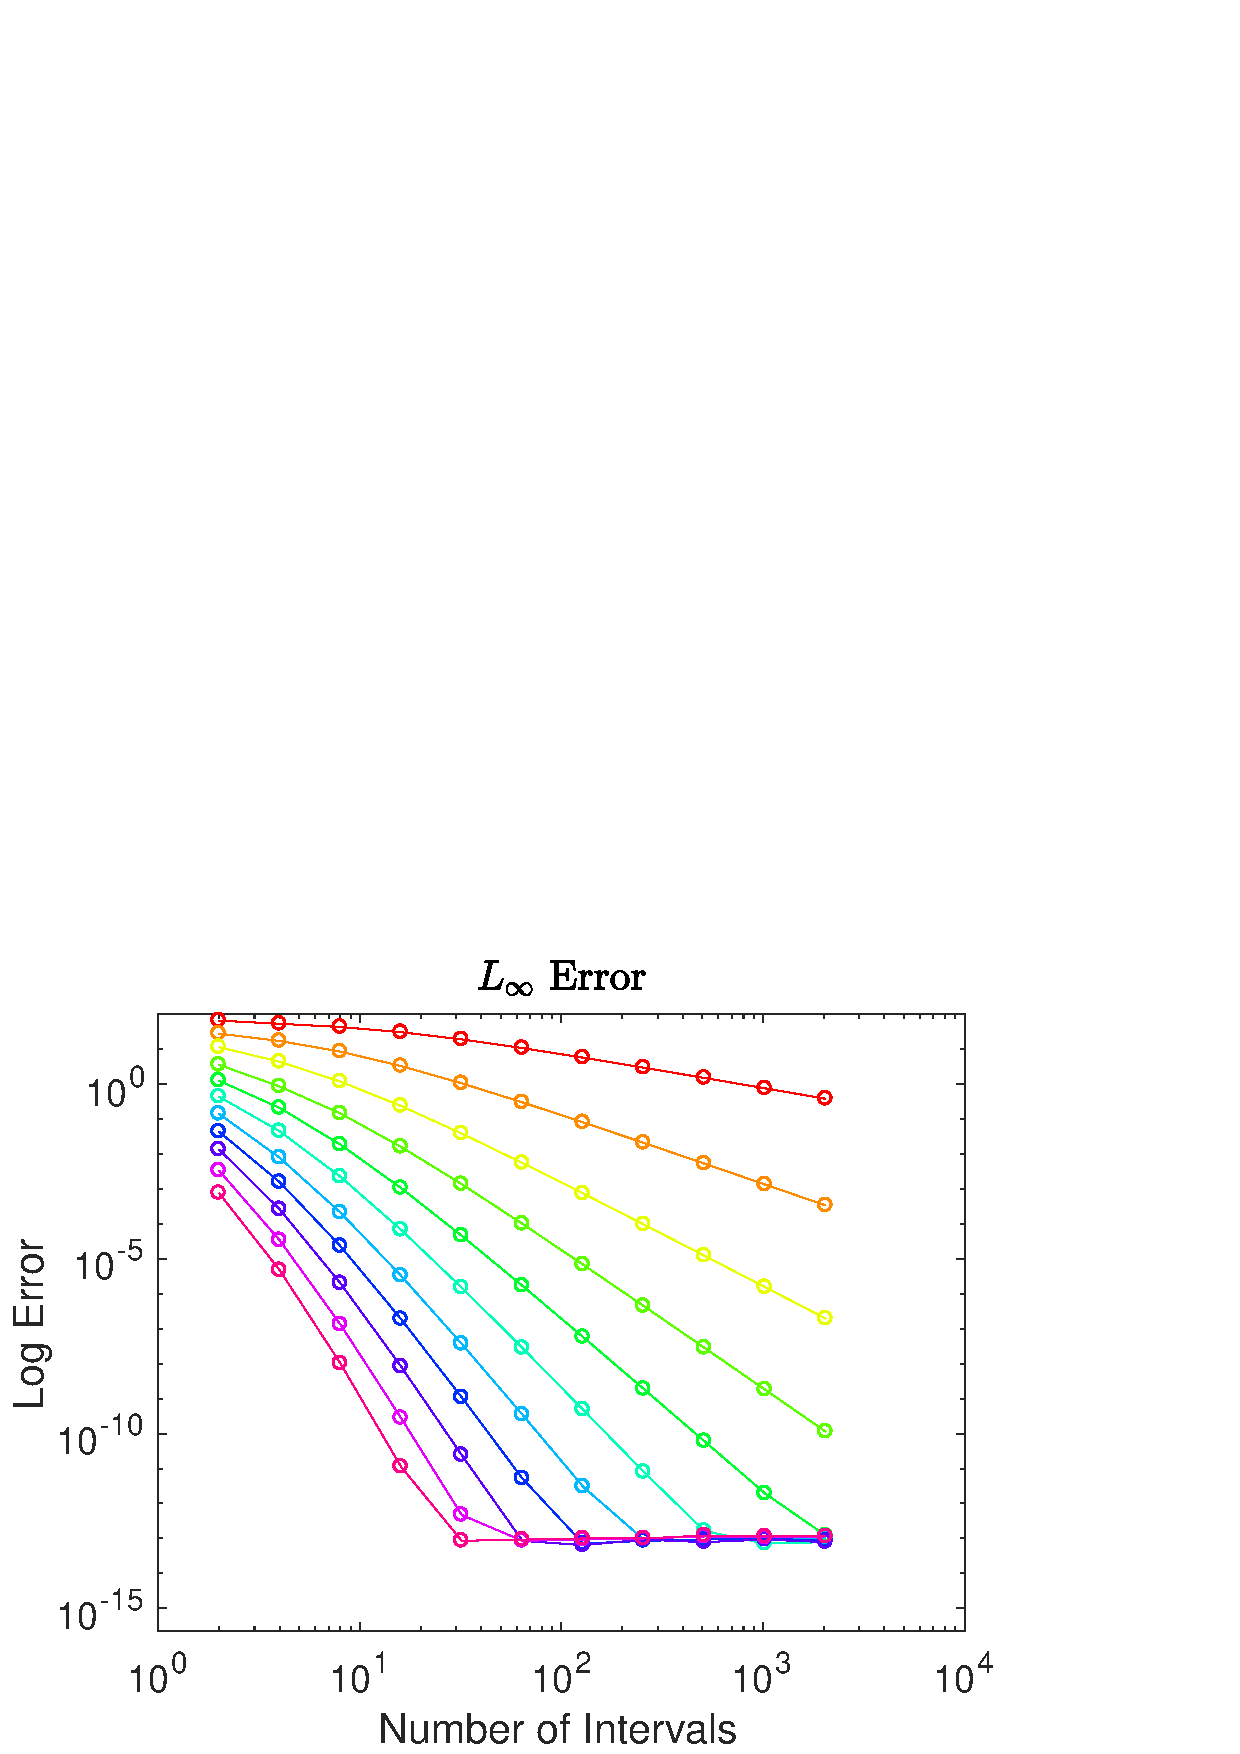
\includegraphics[width=\textwidth]{maxError_0.png}
  \caption{Uniform Norm Error of an Exponential}
  \label{fig:maxErr0}
\end{figure}

\noindent The situation is much the same with respect to the $L_2$ error as depicted below. We see that the $L_2$ error doesn't reach machine precision and yields fewer digits of accuracy compared to the uniform error. 

\begin{figure}[H]
  \centering
  \includegraphics[width=\textwidth]{squareError_0.png}
  \caption{Uniform Norm Error of an Exponential}
  \label{fig:maxErr0}
\end{figure}













\end{document}
